%%%%%%%%%%%%%%%%%%%%%%%%%%%%%%%%%%%%%%%%%
% Large Colored Title Article
% LaTeX Template
% Version 1.1 (25/11/12)
%
% This template has been downloaded from:
% http://www.LaTeXTemplates.com
%
% Original author:
% Frits Wenneker (http://www.howtotex.com)
%
% License:
% CC BY-NC-SA 3.0 (http://creativecommons.org/licenses/by-nc-sa/3.0/)
%
%%%%%%%%%%%%%%%%%%%%%%%%%%%%%%%%%%%%%%%%%

%----------------------------------------------------------------------------------------
%  PACKAGES AND OTHER DOCUMENT CONFIGURATIONS
%----------------------------------------------------------------------------------------

\documentclass[DIV=calc, paper=a4, fontsize=11pt, twocolumn]{scrartcl}   % A4 paper and 11pt font size

\usepackage{lipsum} % Used for inserting dummy 'Lorem ipsum' text into the template
\usepackage[english]{babel} % English language/hyphenation
\usepackage[protrusion=true,expansion=true]{microtype} % Better typography
\usepackage{amsmath,amsfonts,amsthm} % Math packages
\usepackage[svgnames]{xcolor} % Enabling colors by their 'svgnames'
\usepackage[hang, small,labelfont=bf,up,textfont=it,up]{caption} % Custom captions under/above floats in tables or figures
\usepackage{booktabs} % Horizontal rules in tables
\usepackage{fix-cm}   % Custom font sizes - used for the initial letter in the document

\usepackage{sectsty} % Enables custom section titles
\allsectionsfont{\usefont{OT1}{phv}{b}{n}} % Change the font of all section commands

\usepackage{fancyhdr} % Needed to define custom headers/footers
\pagestyle{fancy} % Enables the custom headers/footers
\usepackage{lastpage} % Used to determine the number of pages in the document (for "Page X of Total")

\usepackage[pdftex]{graphicx}
\usepackage{pgfplots}
\usepackage{hyperref}



% Headers - all currently empty
\lhead{}
\chead{}
\rhead{}

% Footers
\lfoot{}
\cfoot{}
\rfoot{\footnotesize Page \thepage\ of \pageref{LastPage}} % "Page 1 of 2"

\renewcommand{\headrulewidth}{0.0pt} % No header rule
\renewcommand{\footrulewidth}{0.4pt} % Thin footer rule

\usepackage{lettrine} % Package to accentuate the first letter of the text
\newcommand{\initial}[1]{ % Defines the command and style for the first letter
\lettrine[lines=3,lhang=0.3,nindent=0em]{
\color{DarkGoldenrod}
{\textsf{#1}}}{}}

%----------------------------------------------------------------------------------------
%  TITLE SECTION
%----------------------------------------------------------------------------------------

\usepackage{titling} % Allows custom title configuration

\newcommand{\HorRule}{\color{DarkGoldenrod} \rule{\linewidth}{1pt}} % Defines the gold horizontal rule around the title

\pretitle{\vspace{-30pt} \begin{flushleft} \HorRule \fontsize{24}{24} \usefont{OT1}{phv}{b}{n} \color{DarkRed} \selectfont} % Horizontal rule before the title

\title{Real-time Sound Feature Construction and Detection for Game Input } % Your article title

\posttitle{\par\end{flushleft}\vskip 0.5em} % Whitespace under the title

\preauthor{\begin{flushleft}\large \lineskip 0.5em \usefont{OT1}{phv}{b}{sl} \color{DarkRed}} % Author font configuration

\author{Ben Schwab, } % Your name

\postauthor{\footnotesize \usefont{OT1}{phv}{m}{sl} \color{Black} % Configuration for the institution name
Duke University, Math 361S Spring 2014 % Your institution

\par\end{flushleft}\HorRule} % Horizontal rule after the title

\date{} % Add a date here if you would like one to appear underneath the title block

%----------------------------------------------------------------------------------------

\begin{document}

\maketitle % Print the title

\thispagestyle{fancy} % Enabling the custom headers/footers for the first page

%----------------------------------------------------------------------------------------
%  ABSTRACT
%----------------------------------------------------------------------------------------


% The first character should be within \initial{}
\initial{T}\textbf{his paper investigates a system to process and identify a set of sound events (specifically whistles and snaps) for use as input to a video game. The environment of a game provides unique constraints that requires real time feature generation and recognition. The paper begins with a brief introduction of sound processing, a background on the Fast Fourier Transform - the key numerical method of this paper - followed by a description of the decision pipeline including the audio features generated and the expected features of snaps and whistles.  }

%----------------------------------------------------------------------------------------
%  ARTICLE CONTENTS
%----------------------------------------------------------------------------------------
\tableofcontents

\section{Introduction}

\par The last five years has marked enormous change in how people interact with video games. From the explosion of touch-based smart phone games to more complex technologies like Microsoft's Kinect, users are interacting with games in more natural and immersive manners. Sound based input has historically been a challenging problem because of the computational complexity of obtaining near $100\%$ accuracy required for an enjoyable video game experience. In this paper I propose a limited set of sound input actions: whistles and snaps. The small set allows faster and more accurate recognition than traditional speech based input. In addition, the choice of this input set allows a surprising amount of user control. As whistles have a distinct pitch, they can be mapped to a two-dimensional scalable input (think of a joystick that can move only up and down). Snapping is a binary input that is most similar to pushing a button on a controller.
\par The primary focus of this paper is the construction of a JavaScript library which will generate ``whistle'' and ``snap'' events. The paper can also be used as a frame to introduce the basics of the DFT and it's application to Digital Sound Processing. In the Discussion section, I discuss a proof of concept game where the library will is used. Currently the game, WhistleHero, can be accessed on \textbf{benschwab.github.io}.

\subsection{Identification Pipeline overview}
\begin{figure}[h]
\centering
\includegraphics[width=90mm]{figures/HighLevelPipeline.png}
\caption{High level overview of the identification pipeline.}
\label{overflow}
\end{figure}
A major challenge of this project was establishing a pipeline which would both analyze sound and determine when snaps and whistles occur. Figure one overviews this \textbf{identification pipeline}.  The identification pipeline starts as soon as a stream of audio is established from a user's laptop microphone. The stream is processed in segments in a local context. A set of features such as energy, fundamental frequency, flatness and envelope shape are attached to the sample during this stage. Due to the real-time restriction of generating input for a video game, instantaneous features in both the time and frequency domain are primarily used, however, the pipeline design allows for global features to be analyzed, albeit in a limited manner.
\par To get the frequency information of the input sound (used for generation of the spectral features of the sound sample) I use the famous \textbf{Discrete Fourier Transform}, specifically,  the optimized \textbf{Fast Fourier Transform}  which can switch a signal between frequency and time representations.
\par Finally, after all the features of a sample have been generated, the similarity of the sample is compared to expected feature sets of whistles and snaps which I established via generating features on a controlled dataset. If a similarity threshold is met, a sound event is emitted.

%------------------------------------------------



%------------------------------------------------

\section{Background}
In this section I give a background on digital sound in the time and frequency domains. Experienced readers can skip to section 2.3 where a background on the constraints of a real time JavaScript sound detection engine are discussed.
\subsection{Digital Sound and the Time Domain}
Sound is a longitudinal wave of pressure variations. Figure 2 gives a visual representation of a sound pressure wave. At an instant in time, the ear perceives the wave at some pressure level. A plot of the intensity over time would be a continuous function $s(t)$ recorded by some target such as an ear or microphone. The WebAudioApi used in this paper normalizes the pressure measurements to be between -1 and 1, where -1 represents low pressure and 1 represents high pressure. This system is known as \textbf{Pulse Code Modulation} or \textbf{PCM}.

\begin{figure}[h]
\centering
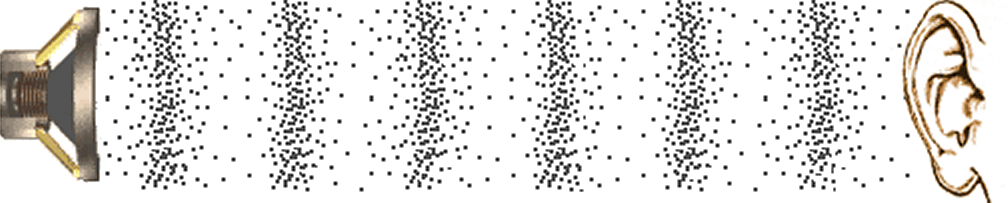
\includegraphics[width=80mm]{figures/pressure_wave.png}
\caption{Sound is the result of high pressure / low pressure variations. [Smuss, 2013]}
\label{overflow}
\end{figure}

\par When a microphone records sound, it records the pressure level at a fixed sampling rate, $ f_s = 1/t_s $ where $t_s$ is how often the sound is sampled. In this project we record at the standard sampling rate of
 $44,100Hz$ or roughly every $t_s =0.02$ milliseconds. This process of converting a continuous signal into a set of discrete values is known as \textbf{quantization}. Figure 3 illustrates the quantization process.

 \begin{figure}[h]
\centering
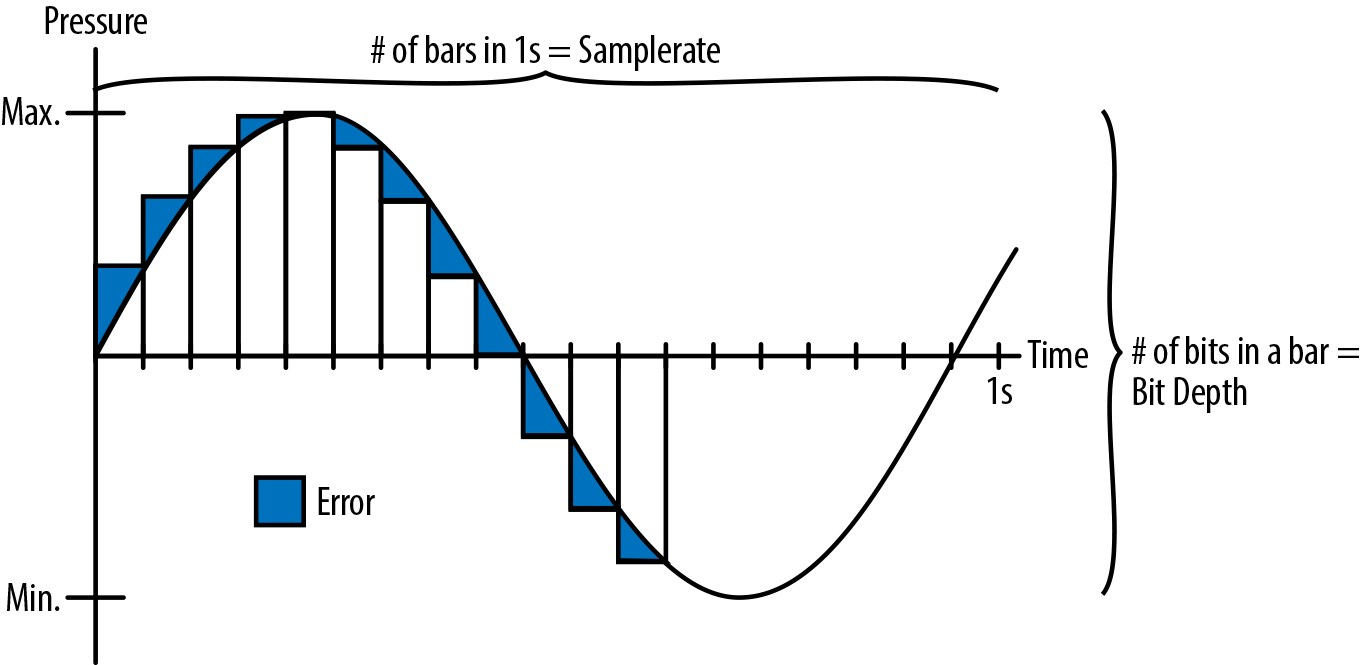
\includegraphics[width=75mm]{figures/quantization.png}
\caption{The quantization process which transforms a continuous sound signal into a discrete array of amplitude values.[Smuss, 2013]}
\label{overflow}
\end{figure}

\begin{figure}[h]
\centering
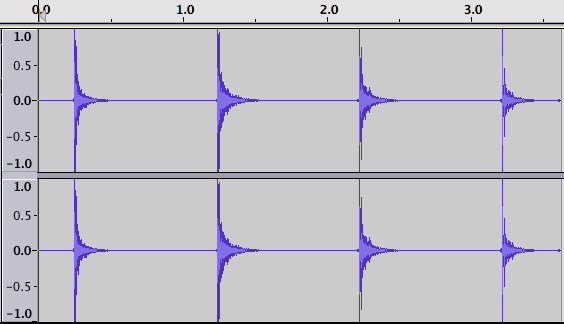
\includegraphics[width=60mm]{figures/snap_timedomain.png}
\caption{The time domain of four finger snaps.}
\label{overflow}
\end{figure}

These sampled signal values represent the signal in the \textbf{time domain}. The time domain information of four snaps is shown in Figure 4.
\subsection{Frequency Domain}
One of the most powerful features of sound is that it can be modeled as a periodic function in the time domain. A steady tone can be generated by pressure values following the pattern of a sine wave. Depending on the period of the wave, we hear a different ``pitch'' (or, more appropriately, frequency). In a sense, the faster packets of high pressure hit one's ear, the higher the pitch one hears.
\par  In the case of a pure sine wave in the time domain, we could imagine representing the signal in a new \textbf{Frequency Domain} under which it would take on a value, $f(x_f)$. This value would indicate if the sound contains a wave at this frequency. For a simple tone wave, in the frequency domain, it would have a high peak at one frequency, $x_f$, and be zero everywhere else. See Figure 5.

\begin{figure}[h]
\centering
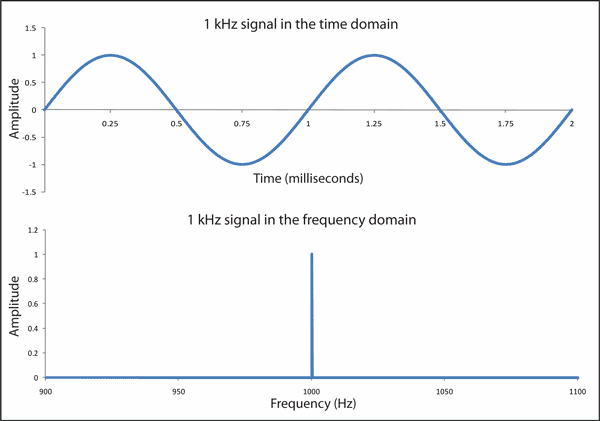
\includegraphics[width=60mm]{figures/twodomains.png}
\caption{An a simple tone converted between time and frequency domains.[Smuss, 2013]}
\label{overflow}
\end{figure}

\par Unfortunately life is not that simple. A sound that can be modeled as a single sinusoid sounds very synthetic. The sounds we hear every day are complex, and fittingly, the signal that represents those sounds look very complex (note the complexity of snaps in Figure 4).

\begin{figure}[h]
\centering
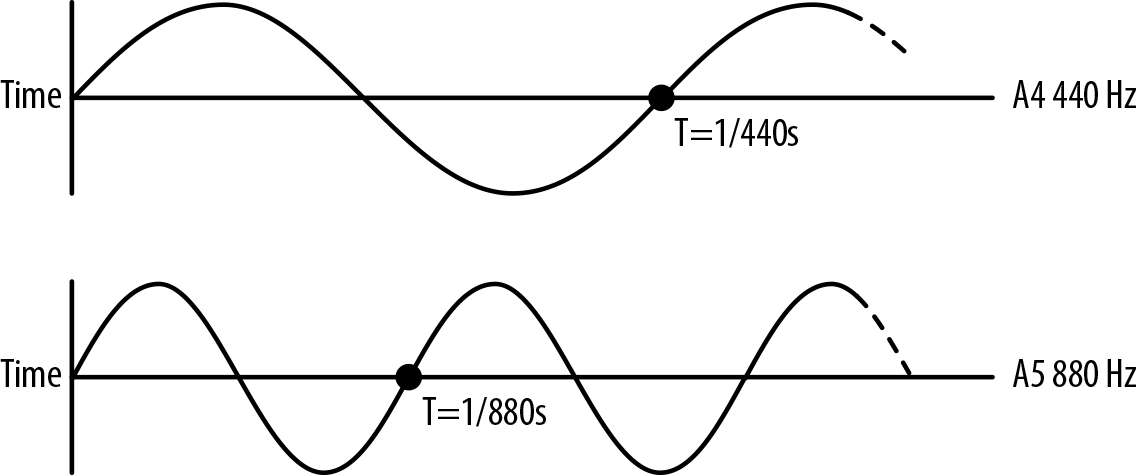
\includegraphics[width=90mm]{figures/PitchGraph.png}
\caption{Two different pure-tone pitches in the time-domain.[Smuss, 2013]}
\label{overflow}
\end{figure}

  However, one of the most beautiful aspects of sound comes from an application of the Fourier Transform. The Fourier Transform states that any function can be represented to an arbitrary degree of accuracy by the sum of cosine and sine functions of varying amplitudes and frequencies. Thus, a complex sound can be represented as the sum of a series of those synthetic ``basic'' sounds which combine to make rich noise. Given a signal in the time domain, the signal can be transformed into a set of trigonometric functions with a meaningful real world interpretation.

\begin{figure}[h]
\centering
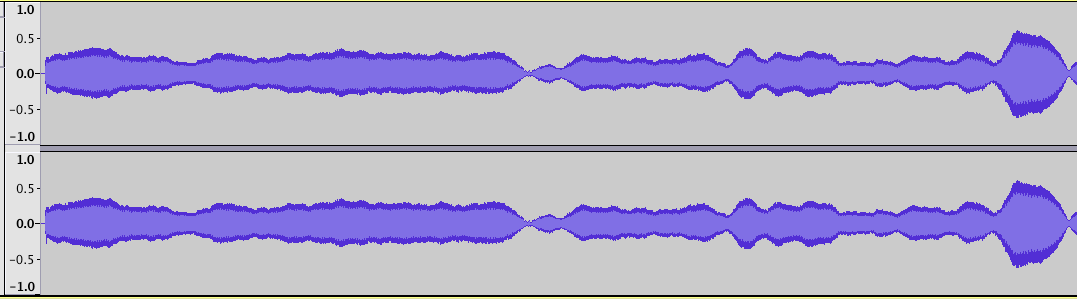
\includegraphics[width=80mm]{figures/whistletimedomain.png}
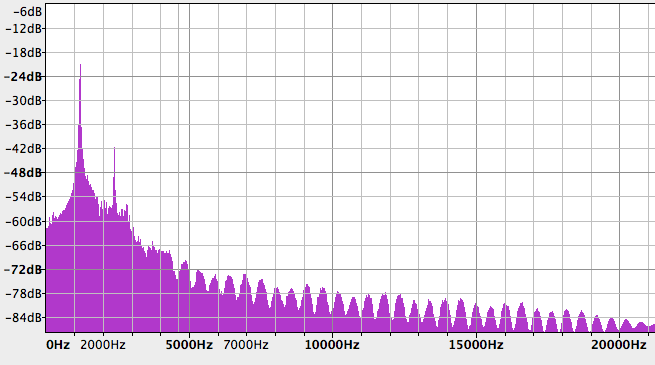
\includegraphics[width=80mm]{figures/frequencydomainwhistle.png}
\caption{A constant whistle signal in the time domain (left) and in the frequency domain(right). The frequency domain clearly reveals that the whistle has a very prominent component at approximately 1200 Hz. Indeed, this is the pitch of the whistle. }
\label{overflow}
\end{figure}

  \par As Figure 7 shows, very useful information about a sound signal is revealed in the frequency domain. The whistle in Figure 7 demonstrates a characteristic shape in the frequency domain, with a distinctive peak at the pitch of the whistle. Generation of features in the frequency domain is known as \textbf{Spectral Analysis}.

\subsection{JavaScript Game Engine Constraints}
JavaScript presents a unique environment to preform active sound input detection due to it's single threaded nature. The following discussion will be at a high-level intending only to frame some of the challenges of using JavaScript to handle Sound Input. Figure 8 shows a representation of JavaScript's single thread. (Sound recording is handled natively through Chrome off the main thread, thankfully.) We receive chunks of approximately 46 milliseconds of sound. Thus, there are 46 milliseconds to fully process the last 46 milliseconds of sound. However, in this 46 milliseconds the game must also render on screen. It does this approximately every 16.6 milliseconds. The game could use some arbitrary portion of the gap between success animation calls to update it's logic. An input engine should allow the maximum about of time possible to be given to the game to compute complex graphical situations. Thus, the engine is written in such a manner that it can detect if the queue of incoming sound is building up. If so it increases its \textbf{hop size} by a factor of 2, effectively cutting processing time in half. See section 4.1.1 for a more in depth explanation of input.
\begin{figure}[h]
\centering
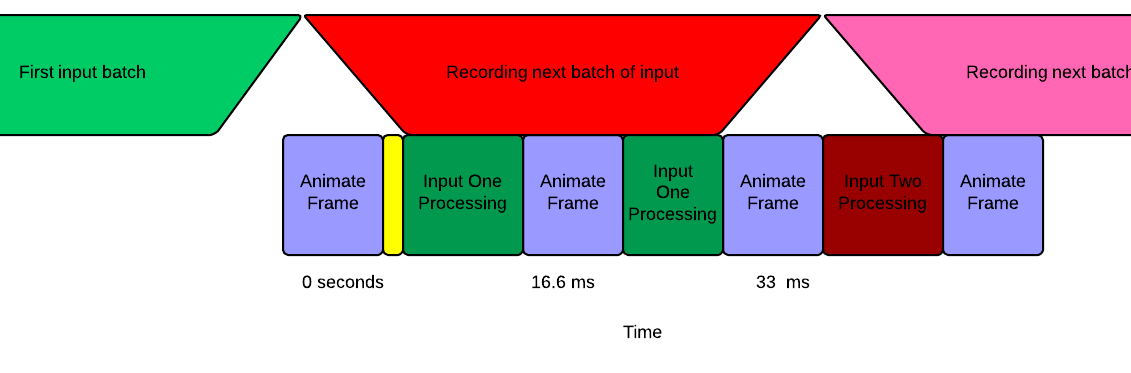
\includegraphics[width=90mm]{figures/JavascriptEventLoop.png}
\caption{JavaScript is single threaded. The sound processing must occur in the windows left open in the game.}
\label{overflow}
\end{figure}

\par The take away from this section is: the Sound Input Engine is guaranteed to  have \textbf{46 ms} of input lag, and often less. The engine will adapt to a heavily computational by decreasing the number of times a sample is processed, which comes at the cost of increasing false negatives.


\section{General Methods}
The primary numerical method of this paper is the FFT. For readers unfamiliar with the FFT, I start this section with a mathematical derivation of the Discrete Fourier Transform and it's practical implementation the Fast Fourier Transform. Experienced readers can skip to section 3.
\subsection{Theory of Fourier Transform*}
\textsubscript{*Adapted from [Sauer, 2012]}
\subsubsection{Mathematical Derivation}

While not strictly necessary for Fourier Transform to function, I will begin the explanation of the FFT by discussing Euler's formula which vastly simplifies the representation of the transform and gives a beautiful geometric interpretation.

\begin{align}
e^{i\theta} = cos(\theta) + isin(\theta)
\end{align}

Equation 1, Euler's formula, is an elegant way to express the set of complex numbers with magnitude equal to one. Figure 9 shows the mapping between the unit circle in the complex plane and Euler's formula.

\begin{figure}[h]
\centering
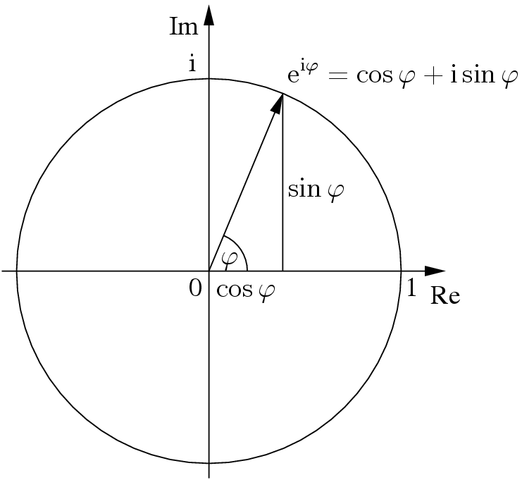
\includegraphics[width=40mm]{figures/EulersFormula.png}
\caption{The connection between the unit circle in the complex plane and Euler's formula. }
\label{overflow}
\end{figure}


Multiplying numbers from Euler's formula is as simple as adding the exponents.

\begin{align}
e^{i\theta}e^{i\gamma} = e^{i(\theta+\gamma)}
\end{align}
Appropriately, this has the geometric meaning that the product of two complex numbers on the unit circle, is another complex number on the unit circle with the new angle the sum of the angles of the factors.
\par We now consider the complex numbers, z, on the unit circle such that $z^n = 1 $. Such complex numbers are known as the \textbf{nth roots of unity}. If a complex number z is $n$th root of unity, but not a $k$th root of unity for any $k<n$, we consider it be a \textbf{primitive nth root of unity}.

\begin{figure}[h]
\centering
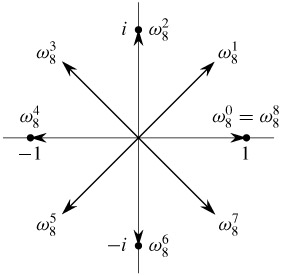
\includegraphics[width=40mm]{figures/eighthroots.jpg}
\caption{The eighth roots of unity. }
\label{overflow}
\end{figure}


Figure 10 shows the 8th roots of unity. It is standard to let $\omega = e^{-i2\pi/n}$ which is always a $n$th root of unity as $\omega^k = e^{-ik2\pi/n}$ which for $k<n$ clearly does not equal one.


The first important statement for the Discrete Fourier Transform is that if $\omega$ is an $n$th primitive root of unity then

\begin{align}
1 + \omega + \omega^2 + \omega^3 + ... + \omega^{n-1} = 1.
\end{align}

This is can be verified with the telescoping sum:

\begin{align}
(1 - \omega)(1 + \omega + \omega^2 + \omega^3 + ... + \omega^{n-1}) = 1 - \omega^n = 0.
\end{align}

As the left factor is not equal to zero, the right factor must be 0. The following equation arrives from the fact that $\omega$ is a $n$th root of unity and the definition of multiplication of complex numbers:

\begin{align}
1 + \omega + \omega^{2n} +  ... + \omega^{n(n-1)} = 1 + 1  ...+ 1 = n.
\end{align}

We can combine these two equations to get:


\begin{align}
\sum_{j=0}^{n-1}\omega^{jk} = \left\{
   \begin{array}{ll}
      n  & \mbox{if } k/n \mbox{ is an integer }\\
      0 & \mbox{ otherwise }
   \end{array}
\right.
\end{align}

The proof follows below: \\

For any k we can write k as $k = m*n +r $ where $r < n$. Thus we can write $\omega^{jk}$ as: $$\omega^{j*(m*n+r)} = \omega^{jmn}\omega^{jr} $$ However, $\omega^{jmn}=1$ by definition of $\omega$ being a $n$th root of unity. If $n|k$ then $\omega^{jr} = 1$ as $r=0$. In this case, the sum becomes $\sum_{j=0}^{n-1}1=n$ If not then the sum becomes $\sum_{j=0}^{n-1}\omega^{jr}$ for some $r<n$. However, using the same telescope sum trick as done in equation 4, we see that this sum equals zero. This completes the proof.

\par Using this knowledge we can now define \textbf{Discrete Fourier Transform}:

\begin{align}
y_k = \frac{1}{\sqrt{n}}\sum_{j=0}^{n-1}x_j\omega^{jk}.
\end{align}

It is useful to define the Fourier Matrix, $F_{n}$, of degree n as:

\begin{align}
 (1/\sqrt n)
 \begin{pmatrix}
  \omega^0 & \omega^0 & \omega^0 & \cdots & \omega^0 \\
  \omega^0  & \omega^1 & \omega^2 &  \cdots &  \omega^{n-1} \\
   \omega^0  & \omega^2 & \omega^4 &  \cdots &  \omega^{2(n-1)} \\
  \vdots  & \vdots  & \vdots &   & \vdots  \\
  \omega^0  & \omega^{n-1} & \omega^{2(n-1)} & \cdots & \omega^{{(n-1)}^2}
 \end{pmatrix}
\end{align}

When we multiply a vector by the Fourier Matrix we transform a vector of real points into a vector of points in the complex plane.

\par Finally, we note that Fourier Matrix is invertible if we define the inverse Fourier matrix as $F_{n}^{-1}$

\begin{align}
\frac{1}{\sqrt n}
 \begin{pmatrix}
  \omega^0 & \omega^0 & \omega^0 & \cdots & \omega^0 \\
  \omega^0  & \omega^{-1} & \omega^2 &  \cdots &  \omega^{-(n-1)} \\
   \omega^0  & \omega^{-2} & \omega^4 &  \cdots &  \omega^{-2(n-1)} \\
  \vdots  & \vdots  & \vdots &   & \vdots  \\
  \omega^0  & \omega^{-(n-1)} & \omega^{-2(n-1)} & \cdots & \omega^{{-1(n-1)}^2}
 \end{pmatrix}
\end{align}

You can see from equation 6, and visual inspection that this is indeed the inverse of $F_{n}$.
\par In summary in this section we have proved we can take a vector of $n$ points we can use the Fourier Matrix to transform it into a vector of complex points of the same degree, and then the inverse Fourier Matrix to return back into its original form.
\subsubsection{Trigonometric Interpretation}

At this point the Fourier Transform may seem like a valid, but arbitrary transform. The usefulness of the Discrete Fourier Transform for sound processing arises from that fact that it carries a very powerful trigonometric meaning. Consider equation 7, the $k$th term in the transformed sample.
Raising $\omega$ to multiples of a number has the geometric interpretation of a point moving around the unit circle at some constant speed, or frequency. When $k = 1$ $\omega$ moves $1/n$ around the the unit circle per term. Thus, it makes one revolution throughout the sum. Similarly when $k=2$, $\omega$ will make 2 revolutions, and so on. Each term $y_k$ is related to a point moving around the unit circle with frequency proportional to $k/n$. Therefore, $y_k$ will be some complex number related to a periodic function. The complex term can be viewed as the phase, and absolute value the amplitude...

\par \textbf{To be finished in final draft.}


\subsection{Fast Fourier Transform}

The naive Fourier Transform on n points using the Fourier Matrix of degree n requires $O(n^2)$ operations. This makes it's use in GameEngine infeasible unless we sample very few points at a time - but this would result in very few frequency buckets making the whistle output feel very jerky (large discrete steps).

\par \textbf{To be finished in final draft.}


\section{Project Methods and Design}
   This sections contains a more in depth description of the specific methods used for this project. Currently, fairly accurate decisions can
   be made with a few simple features. However, the nature of the pipeline allows for more features to be appended as I approach the final version of the project with no change to pipeline itself.
   \par
   The identification pipeline was partially inspired by the pipeline used in Nilsson's paper of human whistle detection. [Nilsson 2008] It contains 4 main sections: input management, feature generation, feature matching, and output.
\subsection{Input}
The WebAudioAPI exposes microphone data sampled at $44,100Hz$. To deal with the constraints specified in Section 2.3, relatively small chunks of sound are processed at a time. The two main parameters of the Input Process is the \textbf{Frame Size} and the \textbf{Hop Size}.
\begin{figure}[h]
\centering
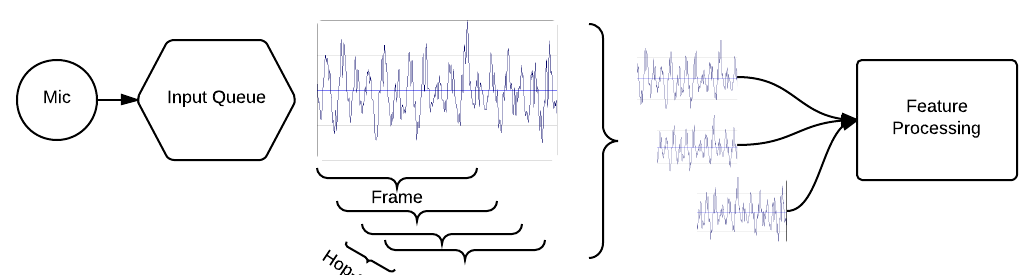
\includegraphics[width=80mm]{figures/InputDiagram.png}
\caption{The input process queue. The sample is retrieved by a window which is moved by a ``hop size'' every iteration.}
\label{overflow}
\end{figure}

The frame size specifies the size the PCM array we will process in a local context for features. Currently the project uses a frame size of 2048 samples.This creates frequency buckets of $10hz$ width, (respectable precision as humans can whistle between 500 and 5000hz [Nilsson 2008]). At this sample rate, 2048 samples is equivalent to $46ms$ of sound.
\par The hop size is the distance the frame is moved when processing the next frame. When the hop size is less than the frame size, portions of samples are reprocessed. The project currently uses a hop size of 256 values, or 5.8ms. Currently, after processing the 2048 values in the frame the first 256 are discarded and 256 more value are appended to the end from the queue. \par I define a new term \textbf{Safe Feature Width}, which is the largest guaranteed feature size that will be processed in a single frame:

\begin{align}
   SFW = WindowFrame - HopSize
\end{align}

Currently, in the project, the SFW is approximately 40ms.

\subsection{Feature Generation}

The input queue passes frames of sound data to the Feature Generator. First the sound frame is processed temporally (no FFT). The temporal processor has the option to normalize the sound sample. If normalization is selected, a \textbf{Peak Normalization} algorithm is used. This algorithm simply scales all PCM values so that maximum value is equal to some target maximum. The project currently normalizes the maximum value to be $0.3$. Peak normalization gives the benefit that it makes peak analysis in the time domain more resistant to a user whistling louder or softer.
\par Next the sample is processed in the Frequency domain. The Spectral Processor performs a FFT on the audio frame, and then attaches a set of spectral features.

\par The following sections contain the current temporal and spectral features generated on a local sample.


\subsubsection{Temporal Features and Relevant Methods}
\subsubsection {Energy}
   The power of a sound signal is defined as:
   \begin{align}
      p_x(n) = |x(n)|^2
   \end{align}
   The energy of a sound signal is defined as:
   \begin{align}
     Energy = \sum_{n=0}^N p_x(n)
   \end{align}
   Therefore, two features attached to a signal that can be computed in $O(n)$ time is the total energy of the signal, and the maximum power of a signal.
   \subsubsection {Peak Detection}
   Peaks are found with a routine that takes the following parameters:
      \begin{itemize}
        \item Number of left and right neighbors the inspected value must exceed to be a peak
        \item Sensitivity - an \textbf{amount} by which the current value must exceed its neighbors by to be a peak (default: 0)
        \item Threshold - a base level which the current value must clear to be a peak (default: 0) \ldots
      \end{itemize}
   \subsubsection {Envelope Analysis}
   Envelope Analysis is currently done through a heuristic which identifies high and medium peaks in the representation of the sound using the Peak Detection routine. These peaks can then be analyzed. One current measure computes the flatness of the envelope.
   \subsubsection{Flatness}
      Flatness is a measure of how ``spiky'' on envelope is. A flat envelope will have a flatness of 1, while a peaked envelope will have a flatness closer to zero.
      \begin{align}
      Flatness = \frac{exp(\frac{1}{N}\sum_{n=0}^{N-1}lnx(n))}{\frac{1}{N}\sum_{n=0}^{N-1}x(n)}
      \end{align}

\subsubsection{Spectral Features and Relevant Methods}
   \subsubsection{Envelope Analysis}
   Again, the Peak Finding routine is run on the FFT information. See Peak Detection and Envelope Analysis in the Temporal Feature section
   \subsubsection{Max Frequency}
   The max frequency is simply the frequency value with largest magnitude.



\subsection{Feature Matcher and Output}
The Feature Matcher has two main routines. Calculate local similarity, and calculate global similarity. This routine only occurs if the signal passes some minimum energy threshold. This is to prevent finding random events in white noise. The user of the library has the option to define functions that will score the local and optional global similarity of the features to whistles and snaps, and the weights used applied to those scores before the value is compared to a final decision threshold. This design was inspired by the perceptron model used in Neural Networking.
\par As noted, the Feature Matcher has a global similarity component. It allows this through a history of the last $n$ decisions and samples.
\par Currently the evaluation functions and thresholds are specified by the user of the library. I currently use a boolean feature presence based approach, and thus the threshold is simply 1 for both whistles and snaps. However, the architecture allows for a more robust similarity test such as using normalized feature vector distance methods.

\begin{figure}[h]
   \centering
   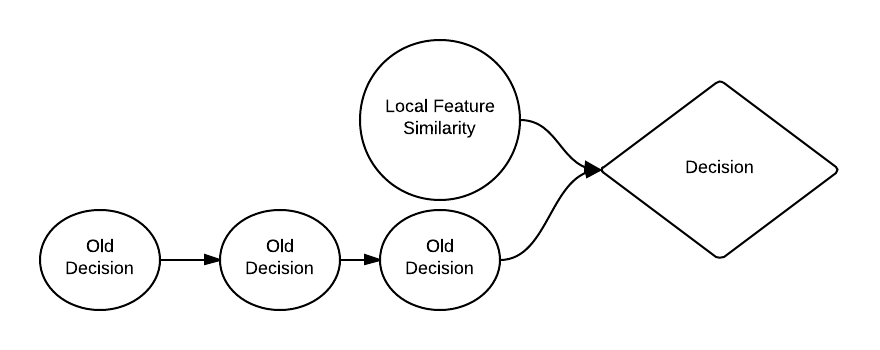
\includegraphics[width=80mm]{figures/FeatureMatcherFuture.png}
   \caption{The feature matcher allows both local similarity and a small about of global context through access to history of previous decisions.}
   \label{overflow}
\end{figure}

\section{Results}
   The Feature Generator in the project attaches a sizable number of features to a sound sample, most in linear time,  (a very small computational foot print). However, accurate classification can actually be accomplished with very few of these features. As the project develops, and possibly in future work, the feature generators will have the algorithms to calculate many \textbf{more} features, but only if the features are actually used in the matcher, will they be calculated. This section discusses the result of running the feature generator on test whistles and snaps. Consistent identification features are then noted.
   \subsection{Features of Whistles}

   Figure 13 shows one frame of a steady whistle in the both in the time domain and frequency domain. The whistle has a relatively constant temporal envelop. Indeed, when the flatness of the envelope was calculated on the samples, it always scored above $0.9$. Whistles typically never had a max energy greater than 0.5, even when the sample contained very loud whistling.
   \par Most of the useful whistle features are found in the frequency domain. A whistle has a single characteristic peak in the frequency domain at its pitch. The vast majority of its spectral content is also between 0 and 10,000hz.


   \begin{figure}[h]
   \centering
   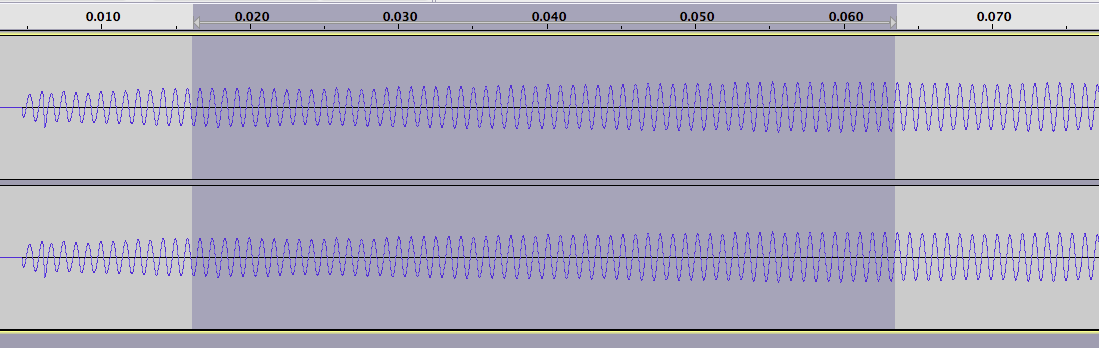
\includegraphics[width=80mm]{figures/whistle_frame_t.png}
   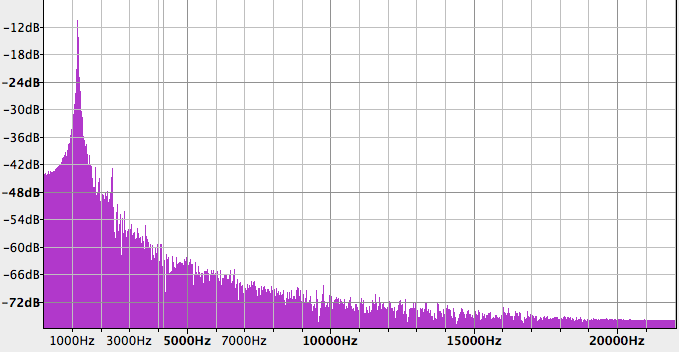
\includegraphics[width=80mm]{figures/whistle_frame_f.png}
   \caption{A 40ms frame of whistle data at attempted constant pitch.}
   \label{overflow}
   \end{figure}
   \par The boolean feature checking routine for a whistle is simple. First the checks requires a temporal envelope with flatness greater than $0.9$. Next it requires that the sound has less than three high peaks frequency peaks, but more than 0. Last it checks to see if the peak is inside the feasible whistle range of $500$ and $5000$ Hz. This process had a near perfect true positive rate. However, it will occasionally trigger from non whistle events, for example if you are playing loud music.

   \subsection{Features of Snaps}

   Snaps are notably characterized by a huge spike of energy in the time domain. Thus, the first feature the boolean snap detecting function checks for is a temporal flatness less then $0.3$. (The vast majority of snaps have a flatness score $<0.01$). Next, it checks that it has a peak energy content greater than $0.8$. Lastly, it verifies that the last sample has a peak energy content less than $.6$. This is to verify that there was a large percussive burst of energy, and as it is infeasible that a user snaps twice in $40ms$, this is a fair assumption. It turns out that these three simple measurements work well for detecting all percussive sounds. In the final version of the project I hope to include more frequency analysis of snaps, as they have a relatively unique spectral envelope.



    \begin{figure}[h]
   \centering
   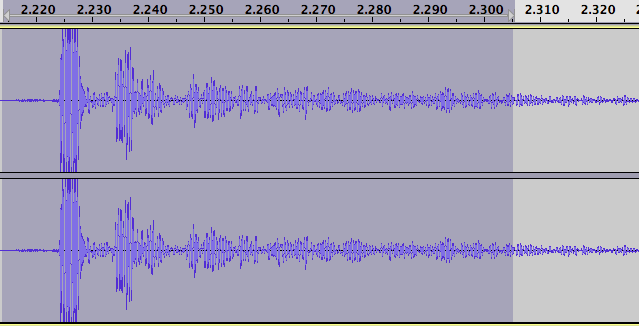
\includegraphics[width=80mm]{figures/snapTimeDomainFrame.png}
   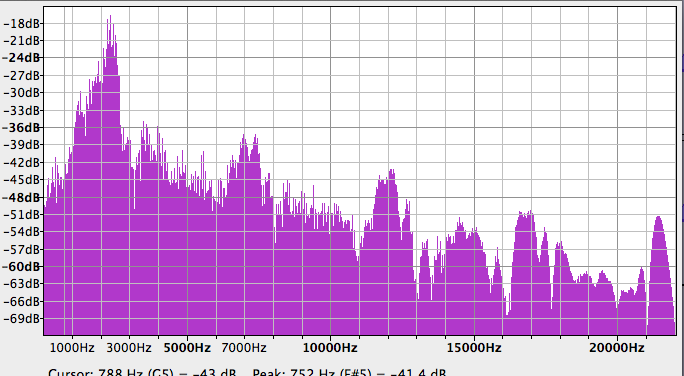
\includegraphics[width=80mm]{figures/SnapFreqDomainFrame.png}
   \caption{A 40ms frame of a snap. }
   \label{overflow}

\end{figure}


\section{Discussion}
   \subsection{Using the API}
      Using the API is as simply as listening for ``SoundInput.detect'' events. You can then switch on the type of input event, and get more details if they exist. As I improve the library games won't have to change any of their code - they will just work better.
   \subsection{Whistle Hero}
   Whistle Hero is demonstration of the API. It assumes no knowledge of how the Audio Processing works besides listening and reacting to snaps and whistles. In the game, a user attempts to ``paint'' a series of circles sliding across the screen with a fixed circular stamp in the center of the screen. The circles are of various sizes, and the user whistles different pitches to match the sizes. When the circles lines up with the central circle, the finger snaps her fingers to make the circle paint the screen. The user is penalized for painting outside the target, but only receives points if the paint hits the target.

    \begin{figure}[h]
   \centering
   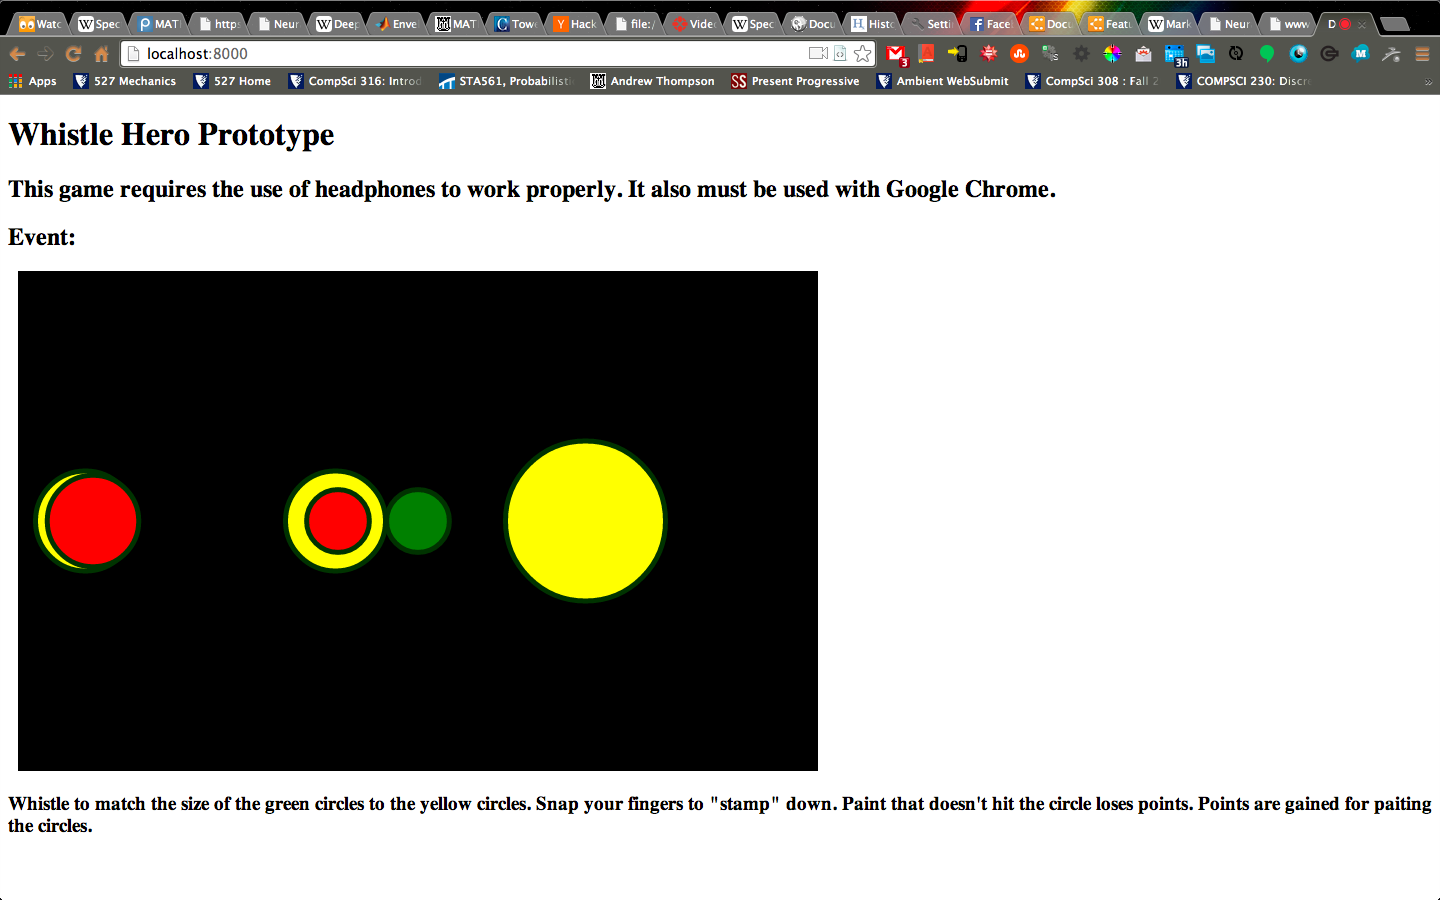
\includegraphics[width=80mm]{figures/whistleheroproto.png}
   \caption{Whistle Hero prototype.}
   \label{overflow}
   \end{figure}

   \par A prototype of the game is on \textbf{benschwab.github.io}, but a lot of the logic has not been implemented. However, whistling and snap detection is demonstrated. (To try the game you must use Google Chrome and have headphones plugged into your computer).

\section{Conclusion}
   In this project I learned a lot about DSP and the FFT, having not been exposed to either extensively in my education to this point. As noted throughout the draft, I intend to make the features system much more robust. Some specific ideas related to the system architecture or noted below.
   \subsection{Future Work}
   \subsubsection{Necessary Feature Specification}
   As I implement more sample features, it may become computationally infeasible to calculate all of them. Thus, the user will be able to specify what features the Matcher will use. The Generator will only produce those features.
   \subsubsection{Custom FFT implementation}
   Currently the project uses a JavaScript implementation of the FFT from \url{<https://github.com/corbanbrook/dsp.js/>}. In the final version I plan to implement my own FFT library so that the project will contain 100 percent custom code.

%----------------------------------------------------------------------------------------
%  REFERENCE LIST

\begin{thebibliography}{99} % Bibliography - this is intentionally simple in this template


\bibitem[Nilsson, 2008]{Nilsson:2008dg}
Nilsson, Bartunek, Nordberg, Claesson. Blekinge Institue of Technology
\newblock {\em Human Whistle Detection and Frequency Estimation}

\bibitem[Peeters, 2004]{Peeters:2004dg}
Peeters. Ircam, Analysis/Syntehsis Team, Igor Stravinksy.
\newblock {\em A large set of audio features for sound description (similarity and classification) in the CUIDADO project}

\bibitem[Sauer, 2012]{Sauer:2006dg}
Sauer, Numerical Analysis 2nd ed. Pearson Education, Inc.
\newblock {\em The Fourier Transform}, p468--499.

\bibitem[Schwarz, 1998]{Schwarz:1998dg}
Diemo Schwarz, Institu de la Recherche et Coordination Acoustique
\newblock {\em Spectral Envelopes in Sound Analysis and Synthesis}

\bibitem[Smus, 2013]{Smus:2013dg}
Smus, Boris. Web Audio API O'Reilly Media, Inc.
\newblock {\em Fundamentals, Advanced Topics}


\end{thebibliography}

%----------------------------------------------------------------------------------------

\end{document}